\documentclass[11pt]{article}

% Increase main memory size
\usepackage{etex}
\usepackage{morewrites}
\usepackage{multicol}
\usepackage{pgfplots}
\usepackage{tikz}
\usetikzlibrary{external}
\tikzexternalize[prefix=cached_models/]

\usepackage{etex}
\usepackage{morewrites}
\usepackage{enumitem}
\usepackage{float}

\listfiles

\usepackage{amsmath, amssymb, amsthm}
\usepackage{mathtools}
\usepackage{graphicx}
\usepackage{geometry}
\usepackage{array}
\usepackage{booktabs}
\usepackage{float}
\usepackage{verbatim}
\usepackage{fancybox}
\usetikzlibrary{3d}

% Page Layout
\geometry{a4paper, margin=1in}
\setlength\parindent{0pt}
\pgfplotsset{compat=1.18}

% Custom commands
\newcommand{\card}[1]{\lvert #1 \rvert}
\newcommand{\inner}[2]{\left\langle #1, #2 \right\rangle}

\newcommand{\remark}{\subsubsection*{Remark}}

\title{\textbf{Vector Calculus Exercises}}
\author{}
\date{}

\begin{document}

\maketitle

\section*{Chapter 2.1}
\subsection*{Exercise 11}
\textbf{Given the set of points \(\{(x_i, y_i)\}_{i=1}^{n}\), and the function \(f(m, b)\) defined as:}
\[f(m, b) = \sum_{i=1}^{n} (y_i - mx_i - b)^2,\]

\textbf{Minimize \(f(m, b)\) using the method of least squares to find the best fit line \(y = mx + b\) for the given data points.}
\vskip 0.5cm
We first compute the partial derivatives of \(f(m, b)\) with respect to \(m\) and \(b\), and set them to zero to find the critical points.:
\[\frac{\partial f}{\partial m} = -2 \sum_{i=1}^{n} x_i (y_i - mx_i - b) = 0,\]
\[\frac{\partial f}{\partial b} = -2 \sum_{i=1}^{n} (y_i - mx_i - b) = 0.\]

Solving the second equation for \(b\) gives:
\[b = \frac{1}{n} \sum_{i=1}^{n} y_i - m \frac{1}{n} \sum_{i=1}^{n} x_i = \bar{y} - m \bar{x},\]

where \(\bar{x}\) and \(\bar{y}\) are the means of the \(x_i\) and \(y_i\) values, respectively. Substituting this expression for \(b\) back into the first equation, we can solve for \(m\):
\[-2 \sum_{i=1}^{n} x_i (y_i - mx_i - (\bar{y} - m \bar{x})) = 0.\]

Expanding and simplifying this equation leads to:
\[\sum_{i=1}^{n} x_i y_i - m \sum_{i=1}^{n} x_i^2 - \bar{y} \sum_{i=1}^{n} x_i + m \bar{x} \sum_{i=1}^{n} x_i = 0.\]

Then we can rearrange this to find \(m\):
\[m = \frac{\sum_{i=1}^{n} x_i y_i - \bar{y} \sum_{i=1}^{n} x_i}{\sum_{i=1}^{n} x_i^2 - \bar{x} \sum_{i=1}^{n} x_i}.\]

\pagebreak

Otherwise, we can express \(y_i\) in terms of the best fit line:
\[y_i = m x_i + b,\]

and form the matrix equation:
\[ A \begin{bmatrix} m \\ b \end{bmatrix} = \mathbf{y},\]

where \(A\) is the matrix of \(x_i\) values and a column of ones, and \(\mathbf{y}\) is the vector of \(y_i\) values. 

\begin{multicols}{2}
This is an inconsistent system, although there exists a solution:
\[\begin{bmatrix} \hat{m} \\ \hat{b} \end{bmatrix},\]

such that:
\[\| Y - A\hat{X} \|^2 \leq \| Y - AX \|^2 \quad \text{for all } X,\]

where \(\hat{Y} \in \text{Col}(A)\) and \(Y - \hat{Y} \in (\text{Col}(A))^{\perp}\). 

\columnbreak
\begin{center}
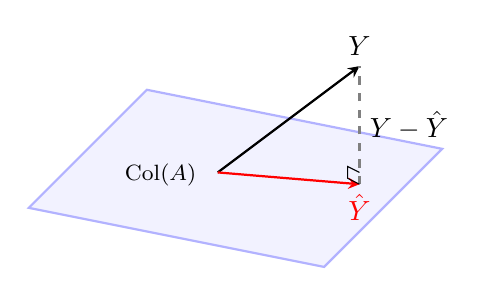
\begin{tikzpicture}[scale=1.5]
    % The Horizontal Plane (Subspace Col A)
    \draw[fill=blue!5, draw=blue!30, thick] (-1,0) -- (1.5,-0.5) -- (2.5,0.5) -- (0,1) -- cycle;
    \node[anchor=south east] at (0.5,0.1) {\footnotesize $\text{Col}(A)$};
    
    \coordinate (O) at (0.6,0.3);
    
    \draw[->, >=stealth, thick, black] (O) -- (1.8,1.2) node[above] {$Y$};
    
    \draw[->, >=stealth, thick, red] (O) -- (1.8,0.2) node[below] {$\hat{Y}$};
    
    \draw[dashed, thick, gray] (1.8,0.2) -- (1.8,1.2) node[midway, right, black] {$Y - \hat{Y}$};
    
    \draw (1.8,0.2) -- (1.7,0.25) -- (1.7,0.35) -- (1.8,0.3);
\end{tikzpicture}
\end{center}

\end{multicols}

Then, \(A = \begin{bmatrix} a_1 & a_2 \end{bmatrix}\) such that 
\[a_i^T (Y - A\hat{X}) = 0 \quad \text{for } i = 1, 2.\]

The expression above can be rewritten as:
\[A^T (Y - A\hat{X}) = 0 \implies A^T Y = A^T A \hat{X} \implies \hat{X} = (A^T A)^{-1} A^T Y,\]

i.e., the normal equations for least squares. Writing
\[F(X) = f(m, b) = \|Y - AX\|^2 = (Y - AX)^T (Y - AX) = Y^T Y - Y^T A X - X^T A^T Y + X^T A^T A X,\]

we can compute the gradient of \(F\) as:
\[\nabla F(X) = -2 A^T Y + 2 A^T A X.\]

Setting \(\nabla F(X) = 0\) gives us the normal equations again:
\[A^T A X = A^T Y \implies X = (A^T A)^{-1} A^T Y.\]

\pagebreak

\subsection*{Exercise 16}
\textbf{Given the function \(h : \mathbb{R}^2 \to \mathbb{R}\) differentiable around \(-1\) such that \(h(-1) = 1\) and, }
\[f(x, y) = h(xy) + 2h\left(\frac{y}{x}\right) - 4, \quad \text{for } x \neq 0,\]
\textbf{find the gradient of \(f\) at the point \((-1, 1)\). Then, obtain the first-order Taylor expansion of \(f\) around the point \((-1, 1)\).}
\vskip 0.5cm
To find the gradient of \(f\) at the point \((-1, 1)\), we first compute the partial derivatives of \(f\) with respect to \(x\) and \(y\). Using the chain rule, we have:
\[\frac{\partial f}{\partial x} = y h'(xy) - \frac{2y}{x^2} \cdot h'\left(\frac{y}{x}\right),\]
\[\frac{\partial f}{\partial y} = x h'(xy) + \left(\frac{2}{x}\right) \cdot h'\left(\frac{y}{x}\right).\]

Evaluating these derivatives at the point \((-1, 1)\), we get:
\[\frac{\partial f}{\partial x}(-1, 1) = 1 \cdot h'(-1) - \frac{2 \cdot 1}{(-1)^2} \cdot h'(-1) = h'(-1) - 2h'(-1) = -h'(-1),\]
\[\frac{\partial f}{\partial y}(-1, 1) = -1 \cdot h'(-1) + \left(\frac{2}{-1}\right) \cdot h'(-1) = -h'(-1) - 2h'(-1) = -3h'(-1).\]

Since \(h'(-1) = 1\), the gradient of \(f\) at the point \((-1, 1)\) is:
\[\nabla f(-1, 1) = \begin{pmatrix} -1 & -3 \end{pmatrix}.\]

The first-order Taylor expansion of \(f\) around the point \((-1, 1)\) is given by:
\[\mathcal{P}_{1, (-1, 1)}(x, y) = f(-1, 1) + \nabla f(-1, 1) \cdot \begin{pmatrix} x + 1 \\ y - 1 \end{pmatrix}.\]

Substituting the values, we have:
\[\mathcal{P}_{1, (-1, 1)}(x, y) = -1 - h'(-1)(x + 1) - 3h'(-1)(y - 1) = -1 - (x + 1) - 3(y - 1)\]

\end{document}